\documentclass[english,a4paper,hidelinks,pdftex, 11 pt, class=report,crop=false]{standalone}
\usepackage[T1]{fontenc}
\usepackage[utf8]{luainputenc}
\usepackage{geometry}
\setlength{\parindent}{0bp}
\usepackage{import}
\usepackage[subpreambles=false]{standalone}
\usepackage{amsmath}
\usepackage{amssymb}
\usepackage{esint}
\usepackage{babel}
\usepackage{tabu}
\usepackage{lmodern}
\usepackage[dvipsnames]{xcolor}
\geometry{verbose, inner=2.3cm, outer=1.8 cm, bmargin=2cm, tmargin=1.8cm}
% Lister med bokstavar
\usepackage{enumitem}

\newcommand{\os}{\\[5pt]}
\newcommand{\vsk}{\\[12pt]}
\newcommand{\net}[2]{{\href{#1}{\color{blue}#2}}}

\usepackage{bm}

\usepackage{hyperref}


\usepackage[many]{tcolorbox}
\newcommand{\reg}[2][]{\begin{tcolorbox}[boxrule=0.3 mm,arc=0mm,colback=blue!3] {\Large \textbf{#1} \vspace{5 pt}}\newline #2  \end{tcolorbox}\vspace{-5pt}}

\newcommand\eks[2][]{\begin{tcolorbox}[boxrule=0.3 mm,arc=0mm,enhanced jigsaw,breakable,colback=green!3] {\Large \textbf{Eksempel #1} \vspace{5 pt}\\} #2 \end{tcolorbox}\vspace{-5pt} }

\newcommand{\asym}[1]{/home/sindre/G/fig/#1}
\newcommand{\fig}[1]{\begin{figure}
		\centering
		\includegraphics[]{\asym{#1}}
\end{figure}}

\newcommand{\ca}[1]{{\color{blue} #1}}
\newcommand{\cb}[1]{{\color{orange} #1}}
\newcommand{\cc}[1]{{\color{ForestGreen} #1}}
\newcommand{\cd}[1]{{\color{cyan} #1}}

\begin{document}
\pagestyle{empty}
\begin{enumerate}[label=(\alph*)]
	\item Kan ein dele parallellogrammet slik at B har større omkrins enn A? Lag ein figur som viser eit eksempel på det. Lag andre figurar som passar til andre svaralternativ.
	\item Kan ein dele parallellogrammet slik at figur A og B har samme areal og omkrins? Viss ja, fins det flerie måtar å gjere det på? Tegn figur.
	\item Del parallellogrammet inn i 3 eller 4 deler der éin av desse er sanne
	\begin{itemize}
		\item delane har lik omrins.
		\item delane har likt areal.
		\item delane har lik omkrins og likt areal. 
	\end{itemize}
\end{enumerate}	
	
\newpage	
\pagestyle{empty}
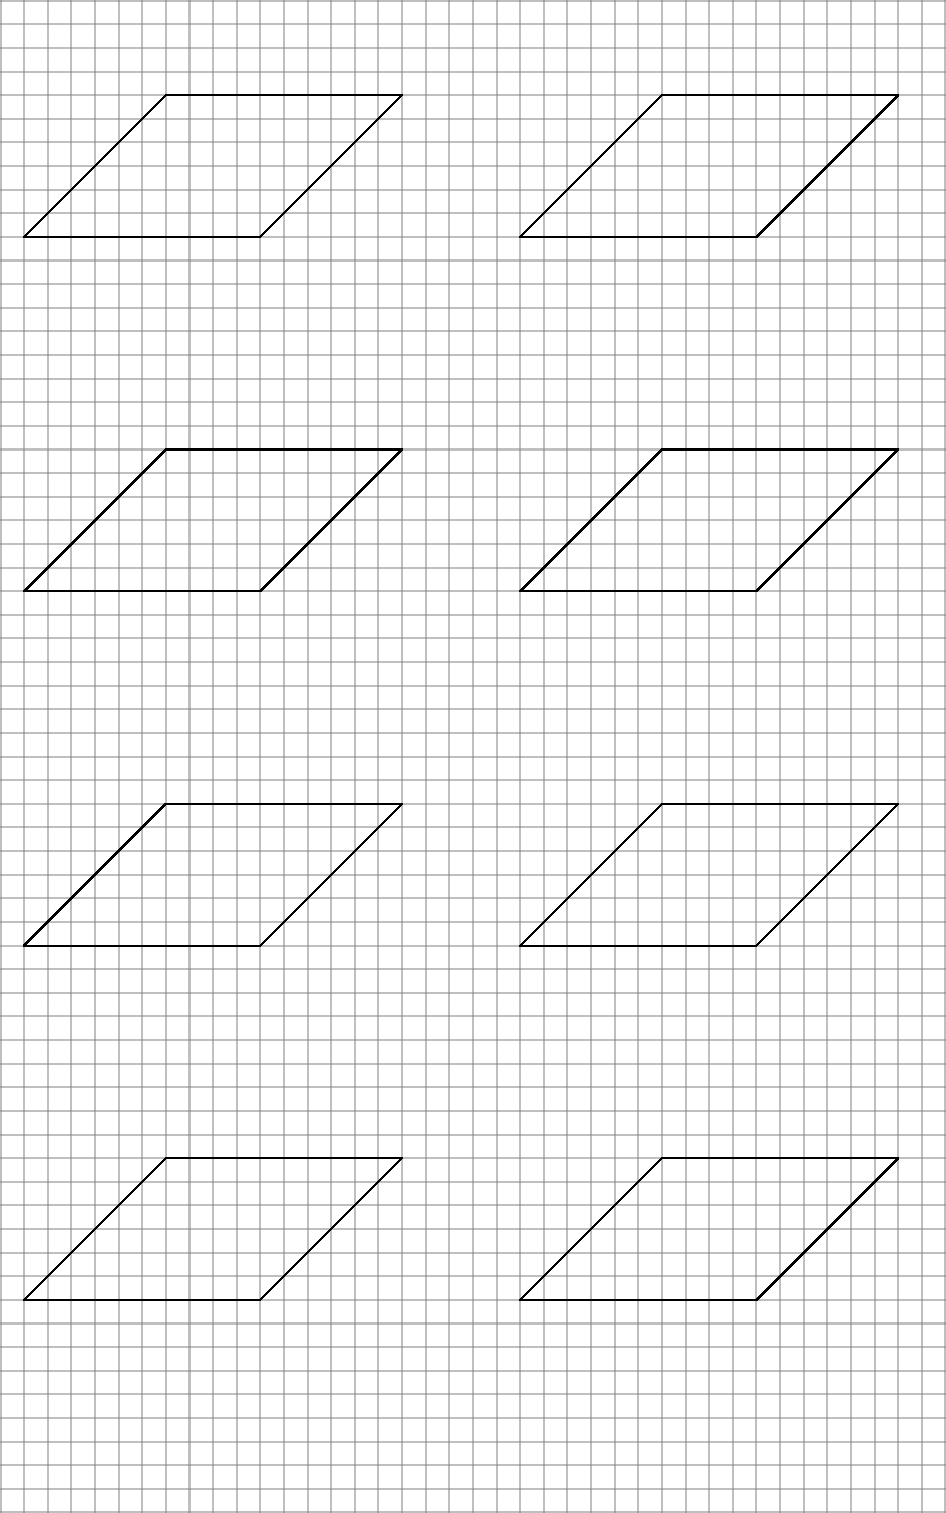
\includegraphics[]{par}

\end{document}


